\section{Electronics and Light Monitoring System}
\subsection{Electronics}

\indent The electronics of the HTCC provide spectrometric and timing information on electron scattering events that are detected by the HTCC within its working acceptance. We need two fast output signals from each channel in order to generate a fast trigger for the CLAS12 spectrometer in experiments with an electron beam. Due to the fact that we need two fast output signals we either had to split the PMT anode signal at some ratio, or we could modify the high voltage passive divider of the PMT by adding a fast preamplifier to generate two identical signals with the same polarity. In many cases the strength (amplitude) of Cerenkov counter signals is smaller than the signal coming from the Minimum Ionizing Particles in the plastic scintillators. Splitting a signal which is already small by itself might be an option depending on the application. \\
\indent In our case we have used modified standard linear passive high voltage divider that is equipped with a fast preamplifier, see Fig.\ref{fig:POPOV_1}.This preamplifier is integrated in the original divider and does not need external power supplies other than the same high voltage power supply that the PMT of a given channel is already using. Amplification coefficient varies from 8 to 10. The preamplifier provides two output signals of negative polarity. 

\begin{figure}[!h]
    \centering
    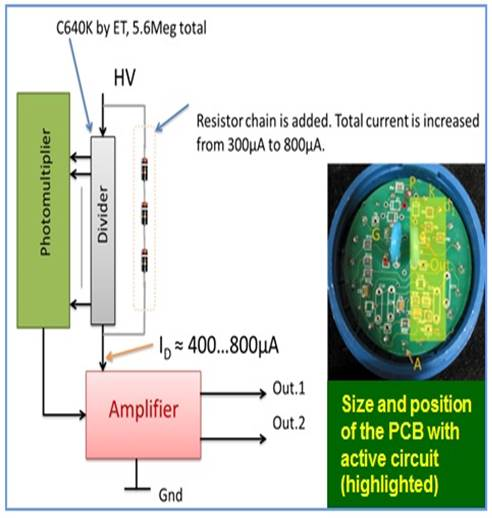
\includegraphics[width=1.0\linewidth,trim={0.0cm 0.0cm 0.0cm 0.0cm},clip]{images/POPOV_1.jpg}
    \caption{Modified high voltage divider with 2 identical outputs}
    \label{fig:POPOV_1}
\end{figure}

The preamplifier is also fast: signal rise time increases by 1.5ns as compared with signal from a passive divider, and it is almost as fast as a signal from fast plastic scintillators. On the Fig.\ref{fig:POPOV_2} and Fig.\ref{fig:POPOV_3} are shown typical signals provided by standard passive divider and by modified divider respectively. The pulses leading edge is about 1.5ns slower than with passive divider and provide near perfect output termination with no signs of any ringing or after-pulsing.

\begin{figure}[!h]
    \centering
    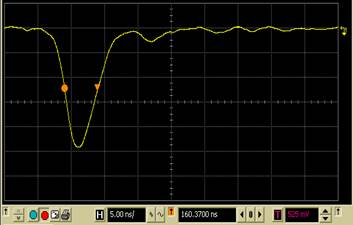
\includegraphics[width=1.0\linewidth,trim={0.0cm 0.0cm 0.0cm 0.0cm},clip]{images/POPOV_2.jpg}
    \caption{Typical output signal provided by standard HV-divider}
    \label{fig:POPOV_2}
\end{figure}

 \begin{figure}[!h]
    \centering
    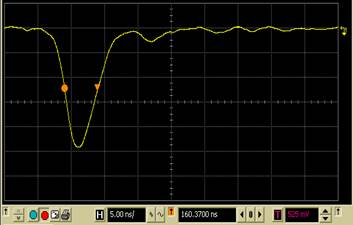
\includegraphics[width=1.0\linewidth,trim={0.0cm 0.0cm 0.0cm 0.0cm},clip]{images/POPOV_3.jpg}
    \caption{Typical output signal provided by modified HV-divider ( with 2 identical outputs}
    \label{fig:POPOV_3}
\end{figure}

The preamplifier is compact, reliable, does not require any changes in the high voltage power supply or in the cabling/connection scheme, consumes relatively low current, and consequently does not need additional cooling. \\
\indent It has to be mentioned that preamplifier we use is generating additional noise as any other preamplifier unavoidably would. Depending on application and components in use the usage of preamplifier might compromise results of PMT gain matching or make them less reliable. In our particular case we use photomultiplier tubes that have a large quartz face-plate that is 5 inches in diameter. Even after selecting PMTs with the lowest possible dark noise and using a standard linear passive divider, designed for the detection of low signals, it was impossible to observe any indication of a single photoelectron peak because photomultipliers were noisy. Measurements of the dark noise were obtained after we developed and used a special dark current measurement procedure that would not require any modification of the standard passive divider. It was important that we were able to avoid using any Nano-Ampere Meters because these meters would necessitate certain modifications to the dividers using positive high voltage. This process allows us to avoid using any meters, and to consequently avoid any changes. Instead of using meters we analyze the dark pulse spectra from the flash ADC, which is triggered by pulse generator. Thus the ratio of integrating the charge to the width of the time window when the charge was obtained provides an accurate and stable estimate of the dark current. On the Fig.\ref{fig:POPOV_4} are shown calibration results for PMT with modified divider.   

 \begin{figure}[!h]
    \centering
    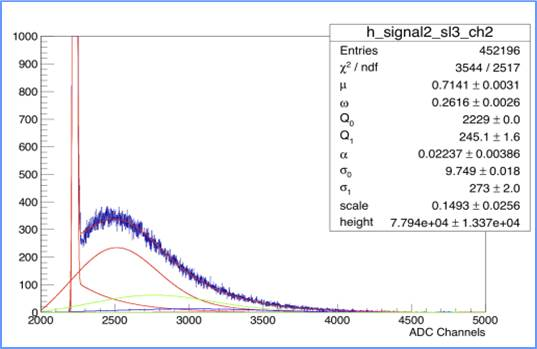
\includegraphics[width=1.0\linewidth,trim={0.0cm 0.0cm 0.0cm 0.0cm},clip]{images/POPOV_4.jpg}
    \caption{Calibration results for PMT with modified divider. In the most cases PMTs have been used at high voltages lower (by about 600 V) than specified for standard divider}
    \label{fig:POPOV_4}
\end{figure}

\subsection{Light Monitoring System and Signal Readout}
\indent
 \\
 \indent In order to run gain matching of all phototubes that do not reveal any single photoelectron signal we developed a new external very fast light source with Light Emitting Diodes. The device is remotely driven, allows for changes in the emitted light intensity, and works at different frequencies in a wide range of these parameters. Once turned on, and after temperature equilibrium is reached, the source is very stable in providing light signals with the required strength and timing. There is an LED panel installed at the entry window of the 4 inch integrating sphere. This panel illuminates the sphere and the light is distributed evenly between fifty coated clear fiber optics that are 1mm in diameter and form a bundle. All the fibers in the bundle have the same length and shine the light directly onto the face of the PMT. The average light intensity is monitored and kept very stable during the entire period of measurements. The average amplitude was at the level of few photoelectrons. Since it is possible to adjust the frequency of the light pulses we were able to observe a corresponding signal from PMT that was well separated from the exponential dark noise. A detailed description of the gain matching is given in the next section. The valuable features of the developed LMS and of procedure for gain matching the phototubes are:
 
 \begin{itemize}
     \item System can be used to calibrate relatively noisy phototubes as well as relatively low noise phototubes
     \item LMS generated calibration light intensity has to be kept stable only during current calibration run (data taking)
     \item It is not necessary to have the fiber optics deliver equal light intensity to any channels, and the calibration of light intensities for different channels have to be only more or less close to each other within 10-20\%
     \item Remarkable repeatability of calibration results even if one uses different setting for the LED source
     \item Maintenance of LMS is essentially simplified since calibration of the LMS itself is not needed
     \item Possible usage of the LMS as often as needed without the necessity of providing the same intensity of light source in different calibration sessions
     \item The LMS can easily be duplicated and successfully used in different places in parallel both in situ and test area
 \end{itemize}

\indent The typical frequency of LED light pulses is in the range of 6 to 10 kHz and is defined by a standard pulse generator. The results obtained during the CLAS12 commissioning run and the following physics run with electron beam have shown that the information provided by JLab proprietary FADC250 modules (Flash ADC) on HTCC signal strength and timing is completely enough to run experiment, with no TDCs used for the HTCC to get timing information. In other words, using just one output signal (without splitting) would be preferable as opposed to the current option where an active high voltage divider provides two identical output signals. One benefit of switching from active to passive dividers would be that one will be dealing with simplified and therefore more reliable high voltage divider. Another valuable benefit would be also a certain reduction of noise in the channels because no more preamplifiers would be in use. We plan to implement corresponding changes.Preliminary comparative tests of two different dividers and same PMT show that the changes will provide higher quality results.